\documentclass{scrartcl}
\usepackage[utf8]{inputenc}
\usepackage[most]{tcolorbox}
\usepackage{tikz}
\usepackage{pgfplots}
\usepgfplotslibrary{groupplots}
\usetikzlibrary{matrix}
\usepackage[T1]{fontenc}
\usetikzlibrary{fit, positioning}
\usetikzlibrary{shapes,arrows}
\usetikzlibrary{positioning, shapes.geometric, calc}
\pgfplotsset{compat=1.18}
\usepackage[most]{tcolorbox}
\usepackage{xcolor}

\begin{document}

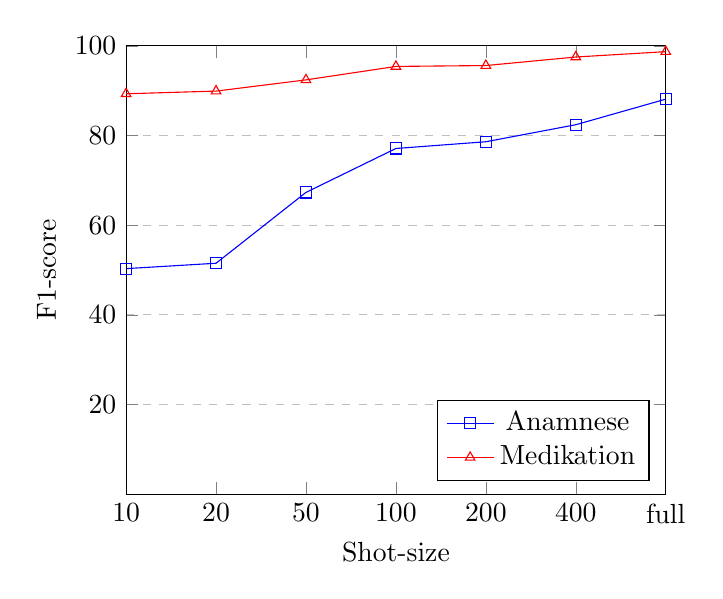
\begin{tikzpicture}
    \begin{axis}[
        xlabel={Shot-size},
        ylabel={F1-score},
        xmin=0, xmax=6, % since you have 7 unique x values (including 'full')
        ymin=0, ymax=100,
        xtick={0,1,2,3,4,5,6},
        xticklabels={10,20,50,100,200,400,full}, 
        ytick={20,40,60,80,100},
        legend pos=south east,
        ymajorgrids=true,
        grid style=dashed,
    ]

    \addplot[
        color=blue,
        mark=square,
        ]
        coordinates {
        (0,50.3)(1,51.5)(2,67.3)(3,77.1)(4,78.6)(5,82.4)(6,88.1) % adjusted x coordinates
        };
        \addlegendentry{Anamnese}

    \addplot[
        color=red,
        mark=triangle,
        ]
        coordinates {
        (0,89.3)(1,89.9)(2,92.4)(3,95.4)(4,95.6)(5,97.5)(6,98.7) % adjusted x coordinates
        };
        \addlegendentry{Medikation}

    \end{axis}
    \end{tikzpicture}

\end{document}